\documentclass{ximera}
\input{../preamble.tex}
\author{}
\license{Creative Commons 4.0 By-NC-SA}
%\outcome{Compute an antiderivative using basic formulas}
\begin{document}
\begin{exercise}
Let $T:\RR^2\rightarrow \RR^2$ be a linear transformation induced by some matrix $A$.  The sketch below shows two lines.  Suppose the following: 
\begin{itemize} 
\item when transformation $T$ is applied to vectors along the line $y=2x$, the vectors reverse direction, but keep their lengths.  
\item when transformation $T$ is applied to vectors along the line $y=-x$, the vectors keep their direction, but triple in length. 
\end{itemize}

 \begin{center}
   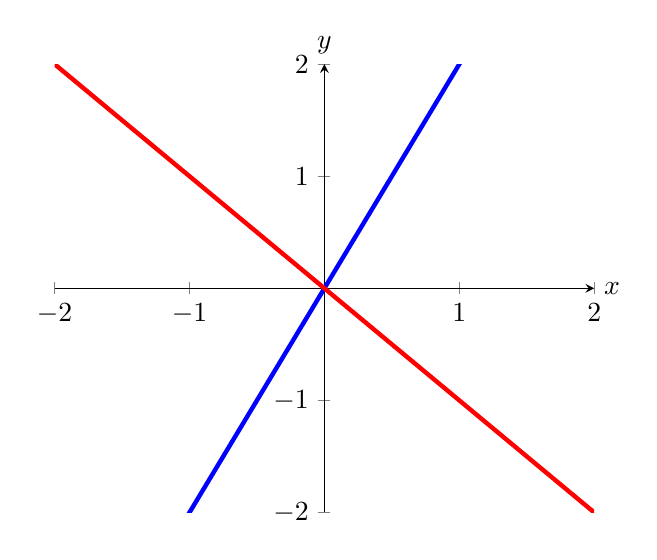
\begin{tikzpicture}  
    \begin{axis}[  
        xmin=-2,  
        xmax=2,  
        ymin=-2,  
        ymax=2,  
        axis lines=center,  
        xlabel=$x$,  
        ylabel=$y$,  
        every axis y label/.style={at=(current axis.above origin),anchor=south},  
        every axis x label/.style={at=(current axis.right of origin),anchor=west},  
      ]  
      \addplot [ultra thick, blue, smooth] {2*x};  
      \addplot [ultra thick, red, smooth] {-x};  
    \end{axis}  
  \end{tikzpicture}  
 \end{center}

Find the eigenvalues of $A$.

$$\text{Eigenvalues of A (in increasing order): }\lambda_1=\answer{-1}, \quad\lambda_2=\answer{3}$$

Find a basis for the eigenspace associated with each of these eigenvalues.

A basis for $\mathcal{S}_{\lambda_1}$: $\left\{\begin{bmatrix}1\\\answer{2}\end{bmatrix}\right\}$

A basis for $\mathcal{S}_{\lambda_2}$: $\left\{\begin{bmatrix}1\\\answer{-1}\end{bmatrix}\right\}$


 \end{exercise}
 
\end{document}